\newcommand*{\Root}{..}
\documentclass[12pt,a4paper]{report}
\usepackage[utf8]{inputenc}
\usepackage[toc,page]{appendix}
\usepackage[english]{babel}
\usepackage[margin=1in]{geometry}
\usepackage[pdftex]{graphicx}
\usepackage{biblatex}
\usepackage{caption}
\usepackage{hyperref}
\usepackage{listing}
\usepackage{listings,lstautogobble}
\usepackage[default,scale=0.95]{opensans}
\usepackage{scrlayer}
\usepackage{setspace}
\usepackage[caption=false]{subfig}
\usepackage{titlesec}
\usepackage{xcolor}

% Custom colors
\definecolor{code-background}{HTML}{EEEEEE}
\definecolor{code-delim}{RGB}{20,105,176}
\colorlet{code-punct}{red!60!black}

% Custom English translations.
\addto\extrasenglish{%
	\def\subsubsectionautorefname{section}%
}

% Configuration for code listings.
\lstdefinelanguage{json}{
	basicstyle=\normalfont\ttfamily,
	numbers=left,
	numberstyle=\scriptsize,
	stepnumber=1,
	numbersep=8pt,
	showstringspaces=false,
	breaklines=true,
	frame=lines,
	backgroundcolor=\color{code-background},
	literate=
	*{:}{{{\color{code-punct}{:}}}}{1}
	{,}{{{\color{code-punct}{,}}}}{1}
	{\{}{{{\color{code-delim}{\{}}}}{1}
	{\}}{{{\color{code-delim}{\}}}}}{1}
	{[}{{{\color{code-delim}{[}}}}{1}
	{]}{{{\color{code-delim}{]}}}}{1},
}


\newcommand\YAMLcolonstyle{\color{red}\mdseries}
\newcommand\YAMLkeystyle{\color{black}\bfseries}
\newcommand\YAMLvaluestyle{\color{blue}\mdseries}

\makeatletter

% here is a macro expanding to the name of the language
% (handy if you decide to change it further down the road)
\newcommand\language@yaml{yaml}

\expandafter\expandafter\expandafter\lstdefinelanguage
\expandafter{\language@yaml}
{
	keywords={true,false,null,y,n},
	keywordstyle=\color{darkgray}\bfseries,
	basicstyle=\YAMLkeystyle,                                 % assuming a key comes first
	sensitive=false,
	comment=[l]{\#},
	morecomment=[s]{/*}{*/},
	commentstyle=\color{purple}\ttfamily,
	stringstyle=\YAMLvaluestyle\ttfamily,
	moredelim=[l][\color{orange}]{\&},
	moredelim=[l][\color{magenta}]{*},
	moredelim=**[il][\YAMLcolonstyle{:}\YAMLvaluestyle]{:},   % switch to value style at :
	morestring=[b]',
	morestring=[b]",
	literate =    {---}{{\ProcessThreeDashes}}3
	{>}{{\textcolor{red}\textgreater}}1     
	{|}{{\textcolor{red}\textbar}}1 
	{\ -\ }{{\mdseries\ -\ }}3,
}


\lstset{
	numbers=left,
	numberstyle=\scriptsize,
	stepnumber=1,
	numbersep=8pt,
	showstringspaces=false,
	breaklines=true,
	frame=lines,
	backgroundcolor=\color{code-background},
	autogobble=true
}

\titleclass{\chapter}{straight}

\titleformat{\chapter}[display]{\normalfont\huge\bfseries}{\chaptertitlename\ \thechapter}{18pt}{\huge}
\titlespacing*{\chapter}{0pt}{20pt}{20pt}

\setcounter{secnumdepth}{5}

% Default values for variables.
\newcommand{\documentdate}{\today}
\newcommand{\documenttitle}{Undefined "documenttitle"}

% Custom macros.
\newcommand{\bolditem}[1]{\item \textbf{#1:}}
\renewcommand{\documentdate}{February 16, 2020}
\renewcommand{\documenttitle}{Progress Report 2}
\begin{document}
\DeclareNewLayer[
foreground,
foot,
contents={\parbox[b][\layerheight][b]{\layerwidth}{%
		
\includegraphics[height=2.5cm]{\Root/.latex-common/logo-ghent-university.pdf}
		\hfill
		
\includegraphics[height=1.2cm]{\Root/.latex-common/logo-sciences.pdf}%
		\vspace*{1cm}
}}
]{titlepage.logos}

\title{
	\vspace*{1.4in}
	\Huge{Thesis (working draft)}\\
	\vspace*{0.4in}
	\Large{\documenttitle}\\
	\vspace*{4cm}
}

\date{\documentdate}
\author{Pieter De Clercq\vspace*{3.5cm}}

\AddLayersToPageStyle{empty}{titlepage.logos}
\maketitle
\RemoveLayersFromPageStyle{empty}{titlepage.logos}
\onehalfspacing
\newpage

\chapter*{Metadata}
\emph{The title of my thesis is still provisionary.}

\begin{itemize}
  \item \textbf{Title:} Applying Test Case Prioritization to optimize Continuous Integrating
  \item \textbf{Name:} Pieter De Clercq \texttt{(01503338)}
  \item \textbf{Study programme:} Master of Science in Computer Science
  \item \textbf{Promotor(s):} prof. dr. Bruno Volckaert, prof. dr. ir. Filip De Turck
  \item \textbf{Supervisors:} Jasper Vaneessen, Dwight Kerkhove
\end{itemize}

\chapter*{Status}
In the previous progress report, I have determined the scope of my masters' thesis. As outlined before, my masters' thesis will research whether or not it is possible to optimize Continuous Integration performance by adopting Test Case Prioritization. In essence, this means that I want to reduce the time occupied by executing regression, integration and unit tests by ranking them according to their failure expectation probability.\\

\noindent First of all, I could not spend as much time to my masters' thesis as I had wanted during December/January, as a result of my busy exam schedule. Since this is my graduation year, I wanted to ensure myself not to fail any exams, a task at which I succeeded. Besides studying however, I was able to find some free moments at which I could progress my thesis.\\

\noindent My first goal was to finish the literature study I had started in the first semester and write a textual report. I have not yet finished this report, however I expect to do so by next week (my textual report currently consists of 21 pages).\\

\noindent Secondly, I had to think of an architecture and start coding an implementation. As to the architecture part, I have devised a simple web-based API as outlined in \autoref{fig:architecture}. I have opted for a web API since this allows data to be exposed easily, optionally for other tools to take advantage of in the future. The architecture works as follows: First, the Continuous Integration system \texttt{[CI-server]} sends a request to the prioritization server \texttt{[PRIO-server]}, indicating that a new commit is ready to be tested. Subsequently, the commit is pulled from the remote repository by the PRIO-server, after which an order is determined. This analysis is performed asynchronously, since it can span several seconds. The CI-server frequently polls the PRIO-server for status updates regarding the analysis. When this is complete, the CI-server receives an order in which the tests should be executed. The tests are executed in the given order and the outcome of the tests is sent back to the PRIO-server as feedback, to improve subsequent analyses. As for the implementation, I have currently finished a proof-of-concept JUnit runner which allows tests (in Java) to be executed in a self-chosen order. The order can currently be provided using a \texttt{YAML}-file, as illustrated in \autoref{lst:order-format}.

\begin{figure}[htbp]
	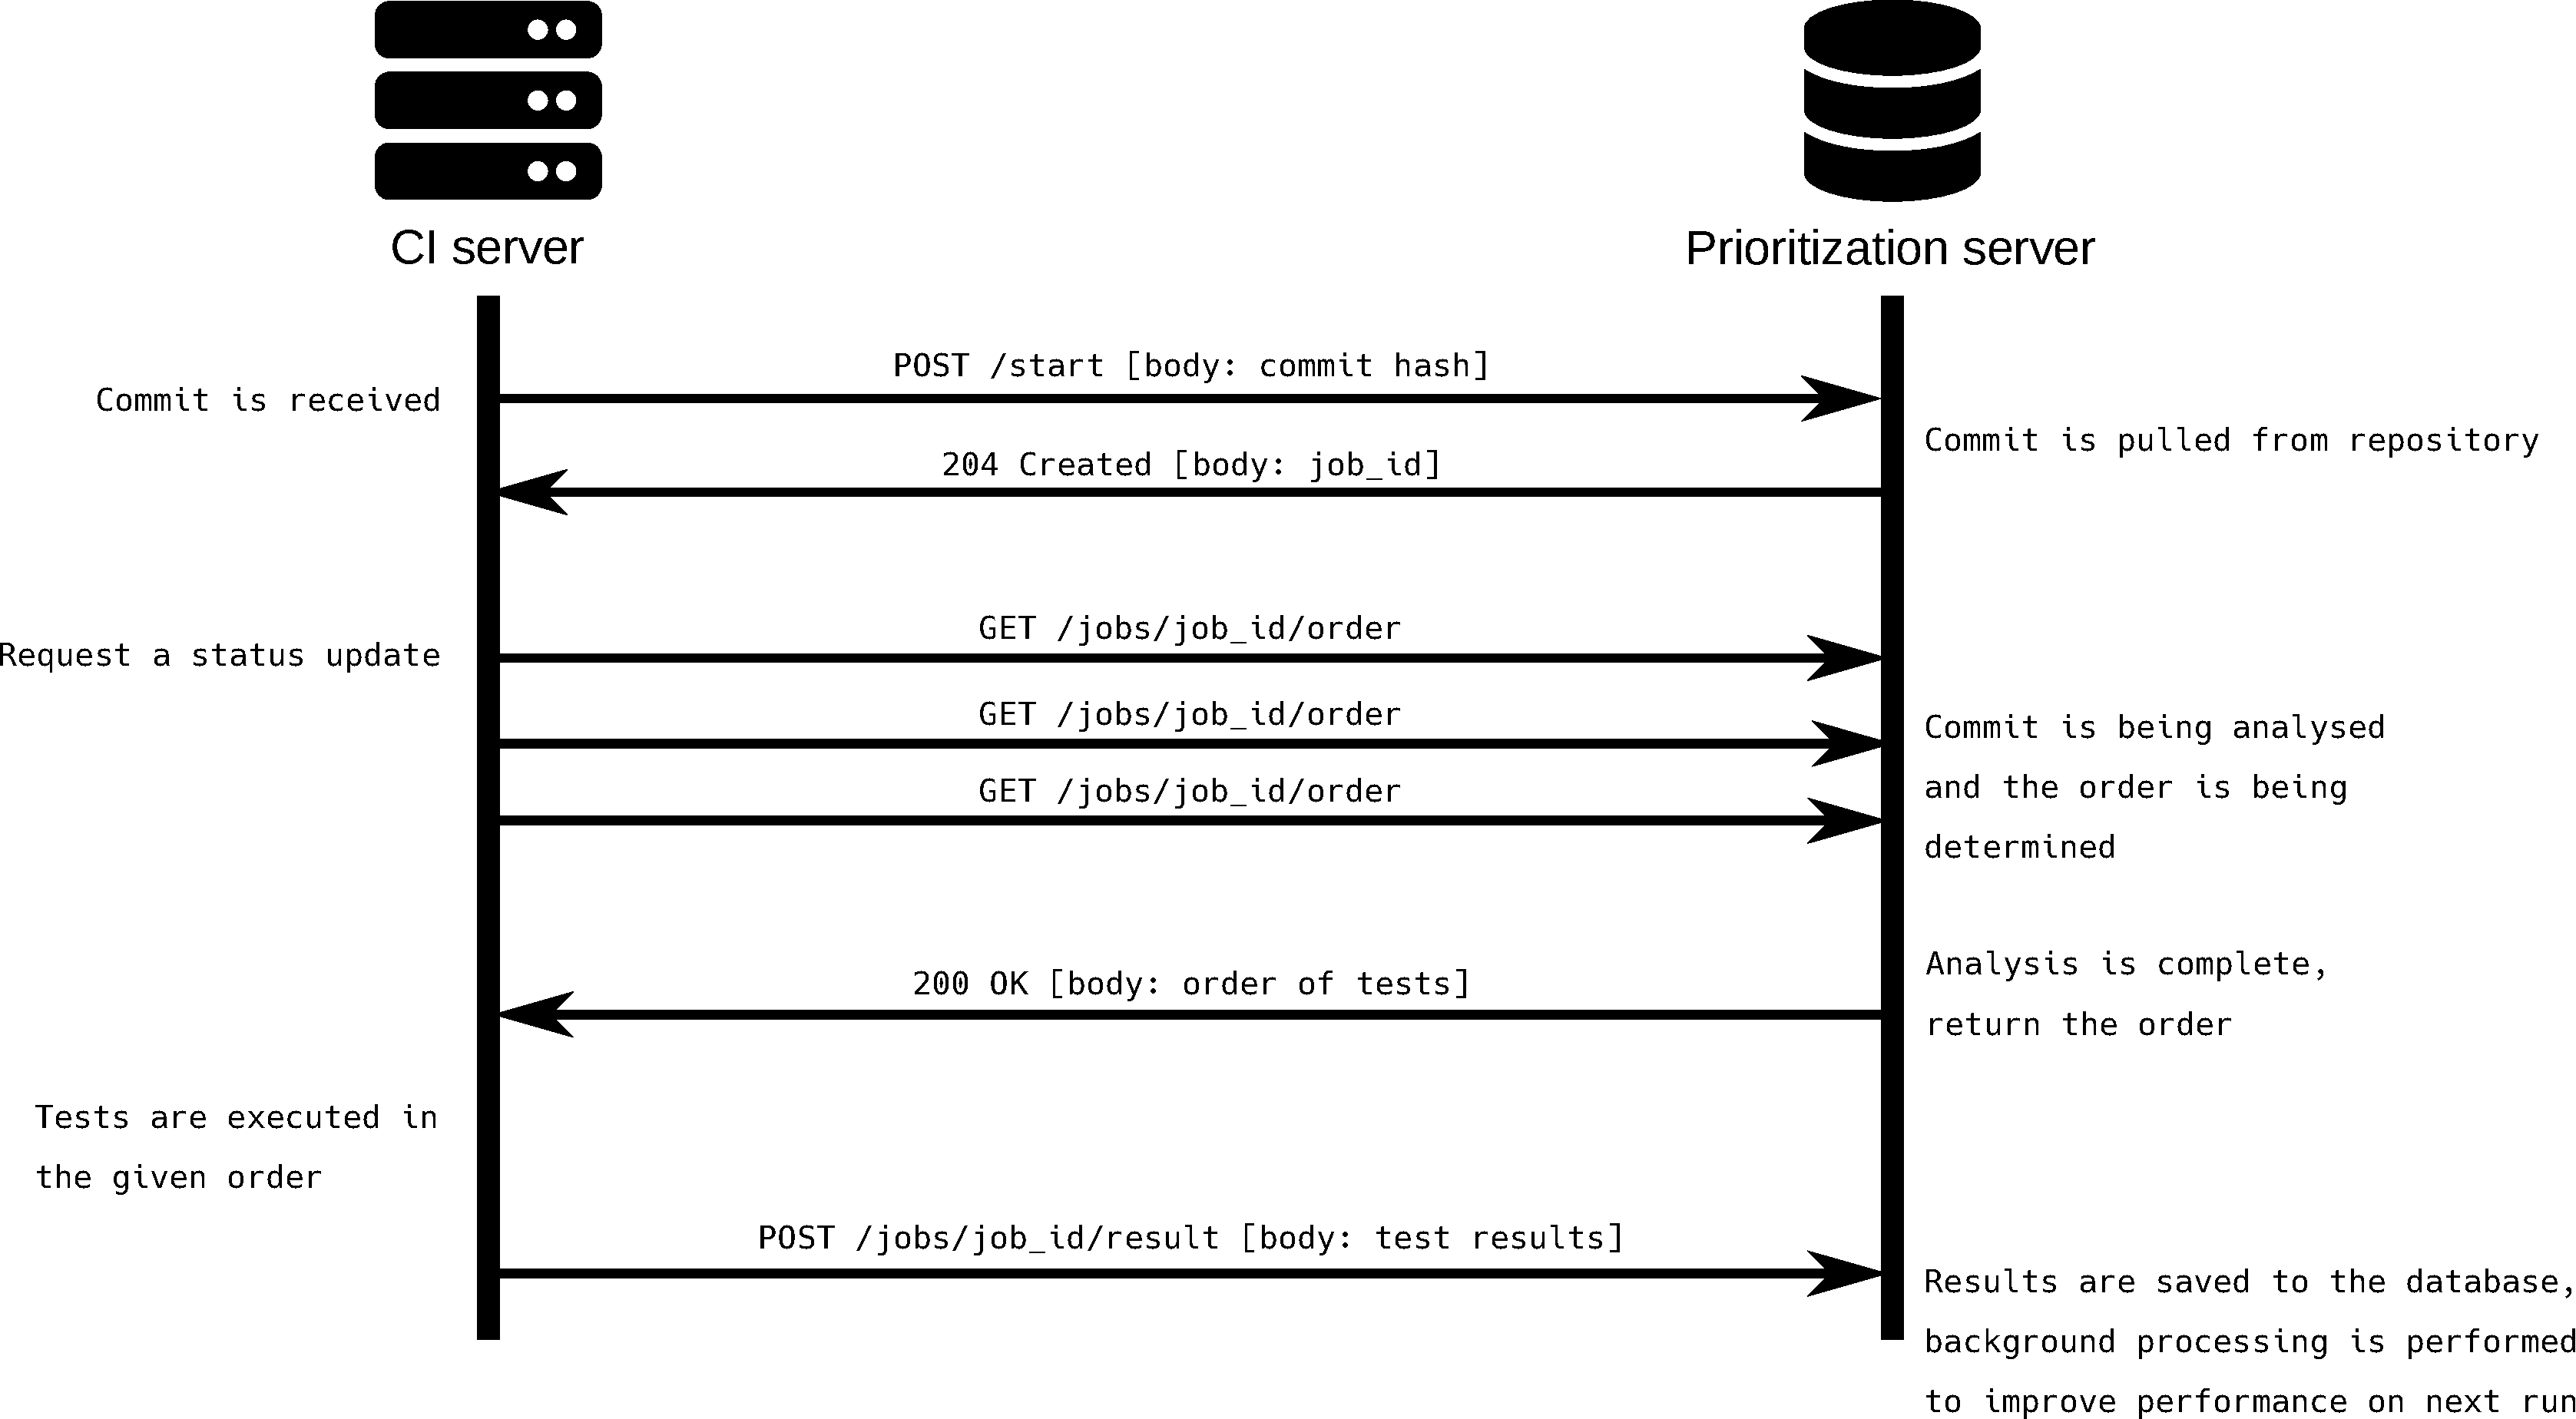
\includegraphics[width=\textwidth]{assets/architecture.pdf}
	\caption{Architecture design of the implementation}
	\label{fig:architecture}
\end{figure}

\begin{lstlisting}[caption=JUnit Order format, label=lst:order-format, language=yaml]
- {class: "FirstTest", method: "testHello"}
- {class: "SecondTest", method: "testWorld"}
- {class: "SecondTest", method: "testLoremIpsum"}
- {class: "FirstTest", method: "testFoo"}
- {class: "SecondTest", method: "testBar"}
\end{lstlisting}

\chapter*{Schedule}
This semester, I only have to attend 1 course, which means that I can dedicate most, if not all of my time towards writing my masters' thesis. Until now I have mainly focussed on writing the textual report, my first task will be to finish the literature study. Starting from next week, I will start implementing the architecture discussed in the previous section. I do not expect the Prioritization server to be very resource intensive (performance testing is however required), so I will attempt to deploy it on a Raspberry Pi. Afterwards, I will feed some open source projects into this architecture, in order to evaluate its performance. In the previous progress report I had already identified three potential projects that I wanted to use. Finally, I will write a detailed report of both the implementation, the results, and future work and append this to the literature study. Concerning these sections, I have already written some schematic pseudo-sentences containing the basic ideas of these sections.\\

\noindent In a final phase, I will investigate the feasibility to support other languages beside Java, and other frameworks beside JUnit, such as Python.

\end{document}
